
\documentclass[a4paper, 12p]{paper} 
\usepackage[margin=2.5cm]{geometry}
\usepackage{amsmath}
\usepackage{graphicx}
\usepackage{lipsum}
\usepackage{xcolor}
\usepackage{booktabs}
\usepackage{float}
\usepackage{subfigure}
\usepackage{titling}
\usepackage{kotex}
\usepackage{gensymb}
\usepackage{threeparttable}

\def\code#1{\texttt{#1}}
\sectionfont{\large\sf\bfseries\color{black!70!blue}}
\date{\vspace{-5ex}}
\renewcommand{\familydefault}{\sfdefault}
\renewcommand{\baselinestretch}{1.3} 

\pretitle{\centering\LARGE\bfseries}
\posttitle{\par}
\preauthor{\begin{flushright}\large}
\postauthor{\end{flushright}}

\title{Frequency Domain Filtering of Gray Images}
\author{전자공학과 20161453 김규래}

\begin{document} 
\maketitle\hrule{}\bigskip

\section{Overview}
이번 과제의 목적은 영상의 fourier domain 특성과, fourier domain 에서의 필터링을 수행해보는 것이다. 디지털 영상에 2D DFT 를 수행함으로써 영상의 fourier domain representation 을 얻어낼 수가 있는데, 이를 통해서 spatial domain 에서는 쉽게 처리하지 못하는 신호들을 어렵지 않게 처리할 수 있다.

\section{Implementation}
언어는 Matlab R2019a 를 사용하였다. Matlab 에서, \code{imshow}, \code{imread}, \code{imagesc}, \code{mag2db}, \code{fft2}, \code{ifft2} 등의 기본 함수들만을 사용하였다. 프로젝트의 디렉토리 구조는 다음과 같다.

\begin{table}[htb]
  \centering
\begin{threeparttable}
  \caption{Synthetic Benchmarks}\label{table:synth}
\begin{tabular}{l|l}
  \toprule
  File                      & Descrition \\
  \midrule
  \code{main.m}             & 구현1, 구현2, 구현3 스크립트를 호출하는 메인 스크립트 \\ 
  \code{impl1.m}            & 구현1 의 스크립트 \\
  \code{impl2.m}            & 구현2 의 스크립트 \\
  \code{impl3.m}            & 구현3 의 스크립트 \\
  \code{center\_freq.m}     & 영상의 spectrum 을 영상 중앙으로 shift 시켜주는 함수 \\
  \code{complex\_image.m}   & 영상의 spectrum, phase 를 반환해주는 함수 \\
  \code{fourier\_filter.m}  & Fourier domain 에서 영상에 필터를 적용하는 함수 \\
  \code{gaussian\_kernel.m} & Gaussian blur kernel 생성 함수 \\
  \code{load\_image.m}      & 이미지를 load 한 다음 $[0, 1]$ 범위로 normalize 하는 함수 \\
  \code{quantize\_image.m}  & 이미지를 8비트로 quantization 해주는 함수 \\
  \bottomrule
\end{tabular}
\end{threeparttable}\\
\end{table}

\subsection{Execution}
Matlab 에서 run.m 을 실행하는 것으로 프로젝트를 실행할 수 있다. 

\subsection{Implementation Remarks}
모든 frequency spectrum, phase angle 영상들은 MATLAB 의 \code{mag2db} 함수를 이용해서 dB 스케일로 리스케일하였다. Fourier domain 영상의 alignment 는 spatial domain 에서 Eq.\ref{eq:centering} 와 같이 phase shift 를 적용해서 수행하였다.

\begin{align}
  \hat{f}(x, y) = f(x, y) \cdot {(-1)}^{(x + y)}\label{eq:centering}
\end{align}

모든 경우에 trailing zero padding 을 적용하였으며, 모든 영상에 대해 2의 승수가 되도록 padding size 를 설정하였다

\subsection{Implementation 1}
구현1 에서는 영상의 Frequency domain representation 에서 frequency spectrum 의 역할과 phase angle 의 역할을 이해하기 위한 것이다. 아래 Fig.\ref{fig:impl1_spectrum} 는 \code{Building.tif}와 \code{Rectangle.tif} 의 frequency spectrum 과 phase angle 을 시각화한 것이다. 

\begin{figure}[H]
\centering
\subfigure[Rectangle.tif] {
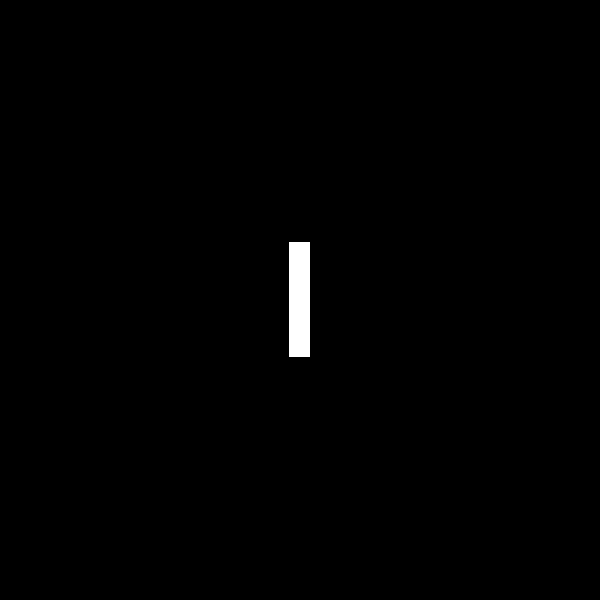
\includegraphics[scale=0.22]{figs/Rectangle.png}
}
\subfigure[Rectangle.tif, Frequency Spectrum] {
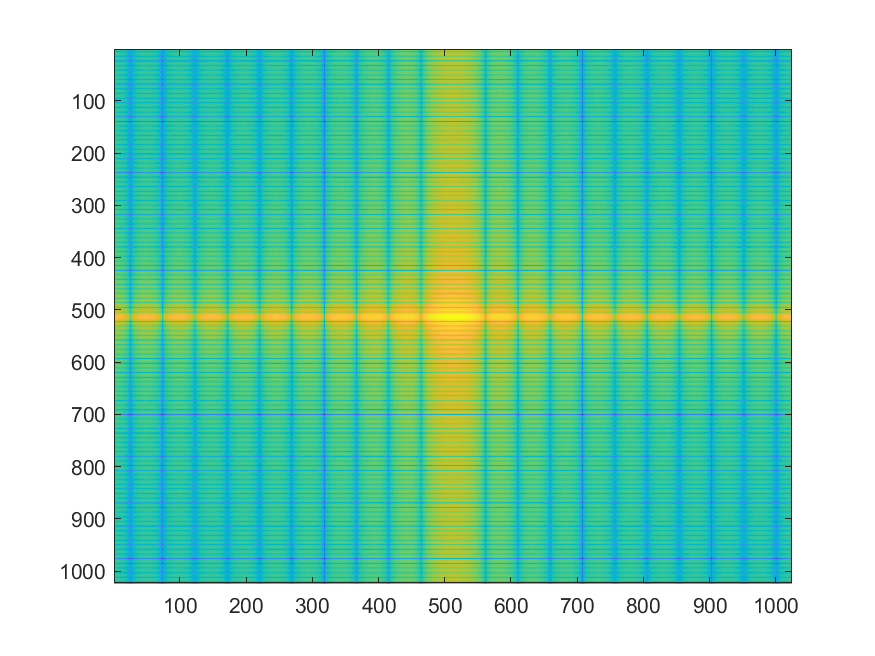
\includegraphics[scale=0.34]{figs/impl1_rec_magnitude.png}
}
\subfigure[Rectangle.tif, Phase Angle] {
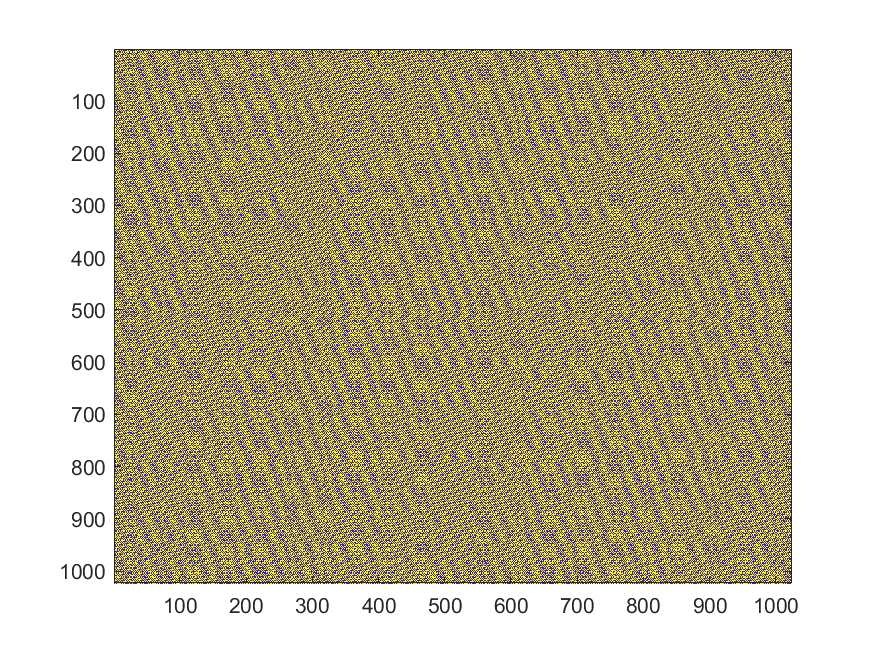
\includegraphics[scale=0.34]{figs/impl1_rec_phase.png}
}
\subfigure[Building.tif] {
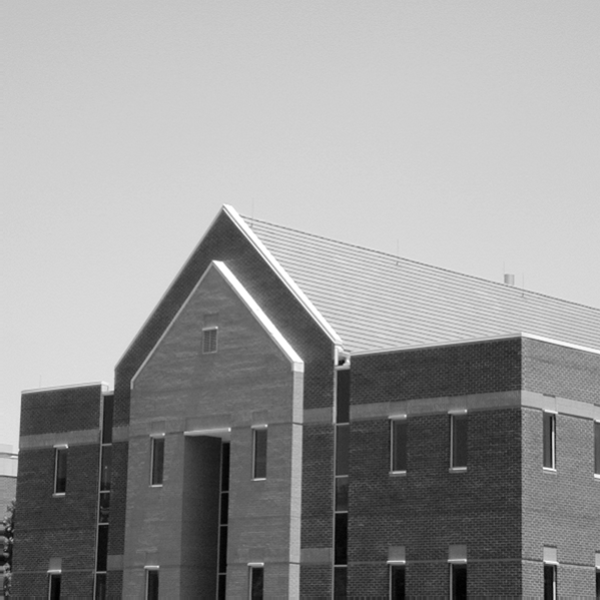
\includegraphics[scale=0.22]{figs/Building.png}
}
\subfigure[Building.tif, Frequency Spectrum] {
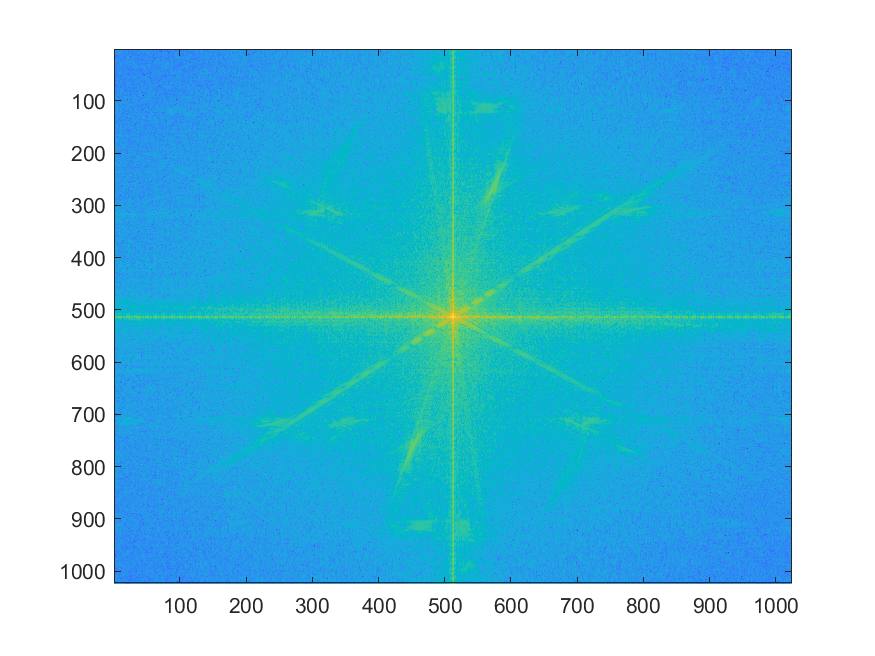
\includegraphics[scale=0.34]{figs/impl1_building_magnitude.png}
}
\subfigure[Building.tif, Phase Angle] {
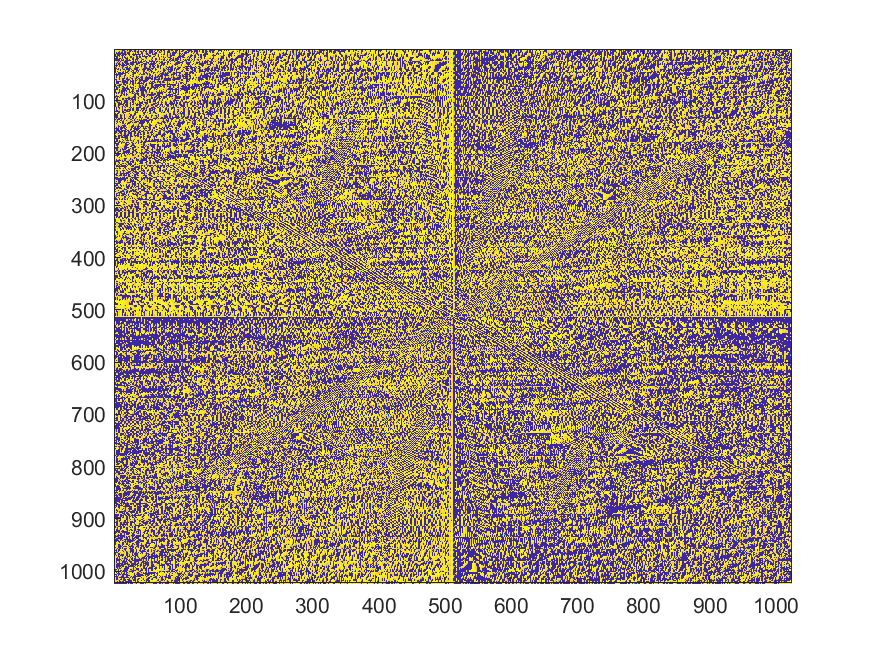
\includegraphics[scale=0.34]{figs/impl1_building_phase.png}
}
\caption{\code{Rectangle.tif}, \code{Building.tif} 의 fourier spectrum image, phase angle image.}\label{fig:impl1_spectrum}
\end{figure}

주파수 도메인의 영상은 Eq.\ref{eq:complex} 으로 표현할 수 있다. 이 때 Frequency spectrum 은 $|\, X(x,y) \, |$, phase angle 은 $\angle{X(x, y)}$ 이 된다.

\begin{align}
  X(x, y) = |\, X(x,y) \, | e^{\, j \, \angle{X(x, y)}}\label{eq:complex}
\end{align}

같은 공식으로, $|\, \hat{X}(x,y) \, |$, $\angle{\hat{X}(x, y)}$ 가 있을 경우 새로운 $\hat{X}(x, y)$ 을 복원해낼 수 있으며, $\hat{f}(x, y) = \mathcal{F}^{-1}[\hat{X}(x, y)]$ 를 inverse fourier transform 을 통해 얻어낼 수 있다. Fig.\ref{fig:impl1_1} 는 이와 같은 방법으로 \code{Building.tif} 의 phase angle, \code{Rectangle.tif} 의 frequency spectrum 으로 복원한 영상이다. Fig.\ref{fig:impl1_2} 는 반대로 \code{Building.tif} 의 frequency spectrum, \code{Rectangle.tif} 의 phase angle 으로 복원한 영상이다.

\textbf{검토사항} Fig.\ref{fig:impl1_1} 의 경우 원래 영상과 다르게 artifact 들이 나타난것을 볼 수 있고, \ref{fig:impl1_2} 에서는 흥미롭게도 \code{Rectangle.tif} 의 형태들이 주기적으로 나타난 것을 볼 수 있다. 이를 통해서 \textit{Phase angle이 영상의 형체 형성에 기여}한다는 것을 예상할 수 있다. 단순히 Phase angle 만을 적용하는 것만으로 원래 영상의 형태를 크게 왜곡시킬 수 있고, 반대로 한쪽의 영상의 형태를 다른 영상에 주입할 수가 있다. \textit{Frequency spectrum (fourier spectrum) 의 경우 영상을 형성하는 성분들을 결정}한다. 따라서 Fig.\ref{fig:impl1_1} 에서는 주파수 성분이 단순하기 때문에 복잡한 형태를 가진 phase angle 을 적용해도 복잡한 형태의 왜곡이 발생하지 않은 것이다.

\begin{figure}[H]
\centering
\subfigure[original] {
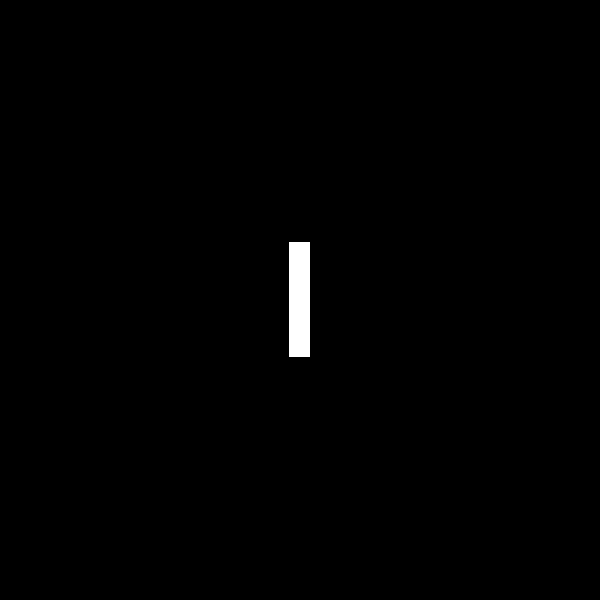
\includegraphics[scale=0.20]{figs/Rectangle.png}
}
\subfigure[reconstructed] {
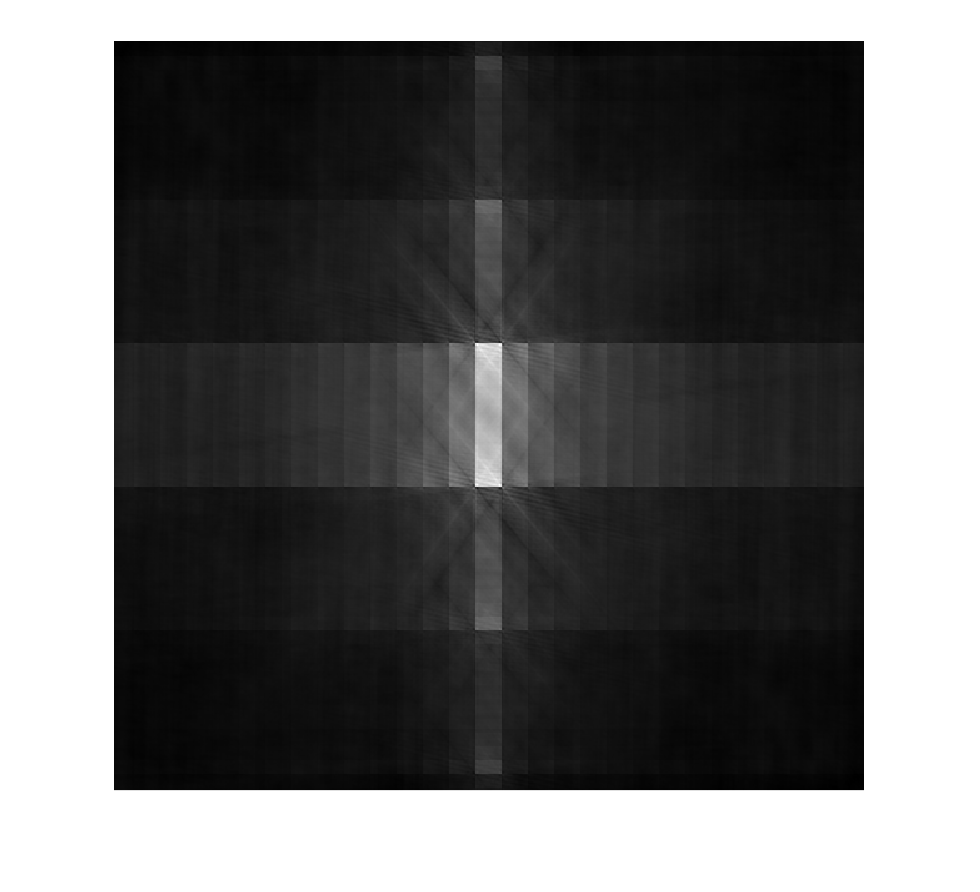
\includegraphics[scale=0.3]{figs/impl1_1.png}
}
\caption{\code{Rectangle.tif} 의 spectrum과 \code{Building.tif} 의 phase angle 을 이용해서 이미지를 복원한 경우.}
\end{figure}\label{fig:impl1_1}

\begin{figure}[H]
\centering
\subfigure[original] {
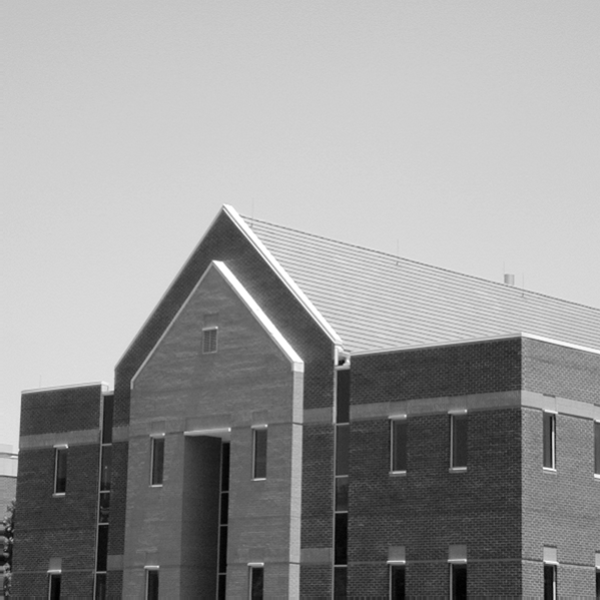
\includegraphics[scale=0.20]{figs/Building.png}
}
\subfigure[reconstructed] {
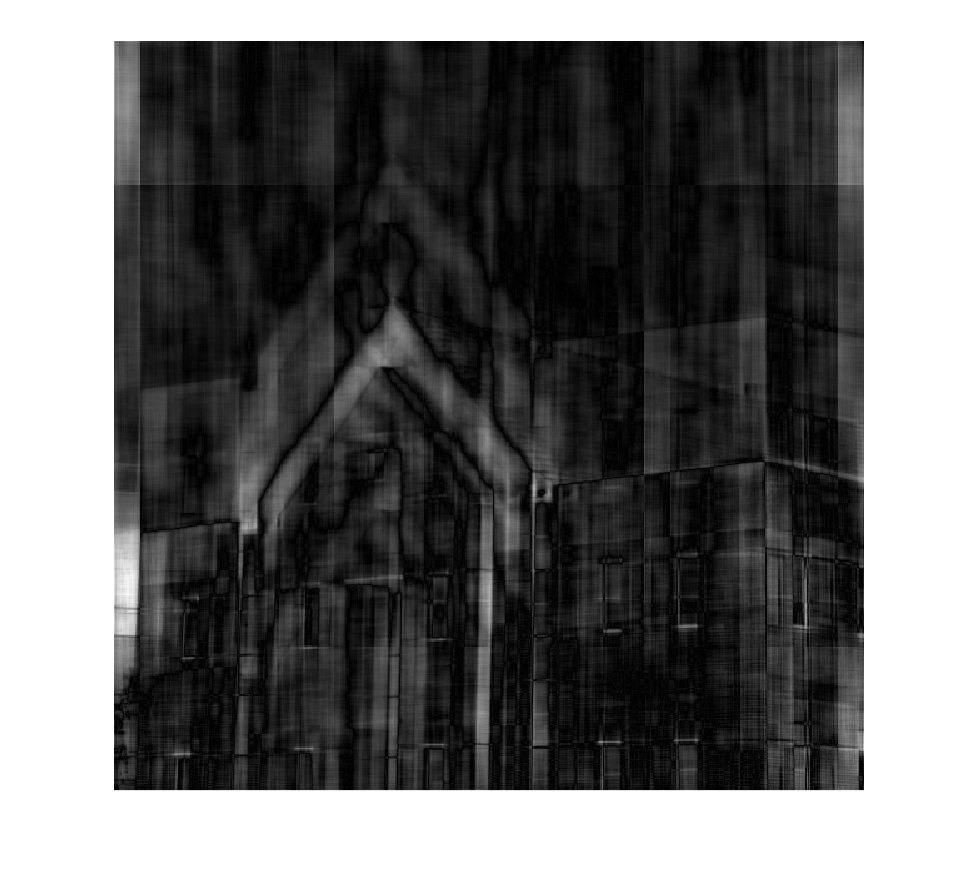
\includegraphics[scale=0.3]{figs/impl1_2.png}
}
\caption{\code{Rectangle.tif} 의 phase angle과 \code{Building.tif} 의 spectrum 을 이용해서 이미지를 복원한 경우.}\label{fig:impl1_2}
\end{figure}

\subsection{Implementation 2}
구현2 에서는 Box filter 와 Gaussian blur 의 frequency domain 특성에 관해서 분석을 하고, 이들을 frequency domain 에서 적용한 결과를 관찰한다.

Fig.\ref{fig:impl2_spectrum} 은 Box filter 와 Gaussian blur 의 Frequency spectrum 이다. 원본 영상을 $f(x, y)$, 필터를 $g(x, y)$ 라 할 때 필터의 적용은 Eq.\ref{eq:filtering} 로 표현할 수 있다.

\begin{align}
 f(x, y) * g(x, y) = \mathcal{F}^{-1}[\, \mathcal{F}[f(x, y)] \circ \mathcal{F}[g(x, y)] \,]\label{eq:filtering}
\end{align}

\begin{figure}[H]
\centering
\subfigure[Box $11 \times 11$] {
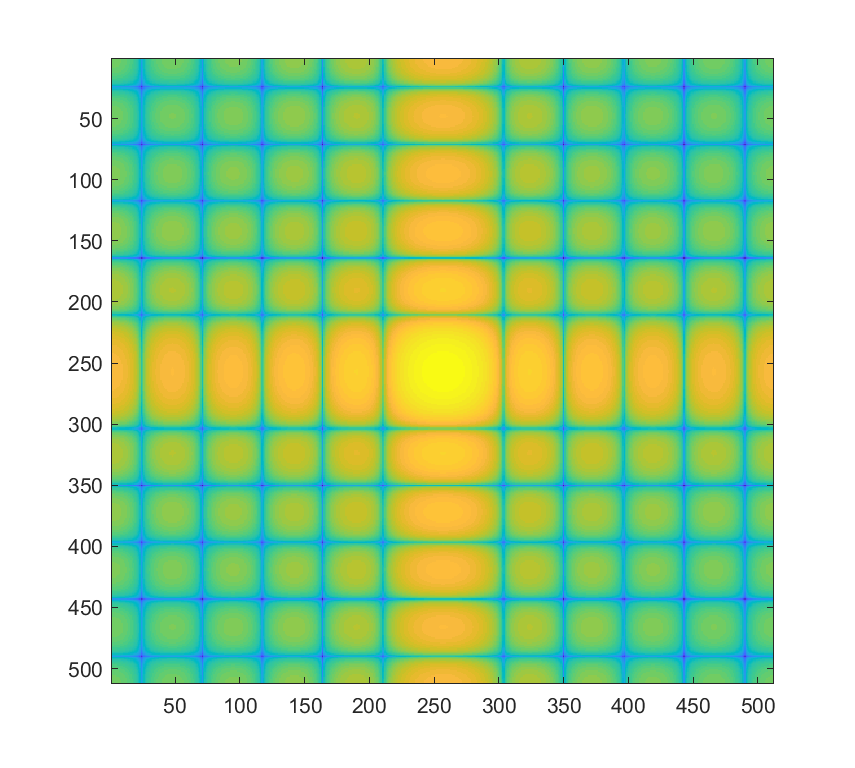
\includegraphics[scale=0.40]{figs/impl2_box1_spec.png}
}
\subfigure[Box $21 \times 21$] {
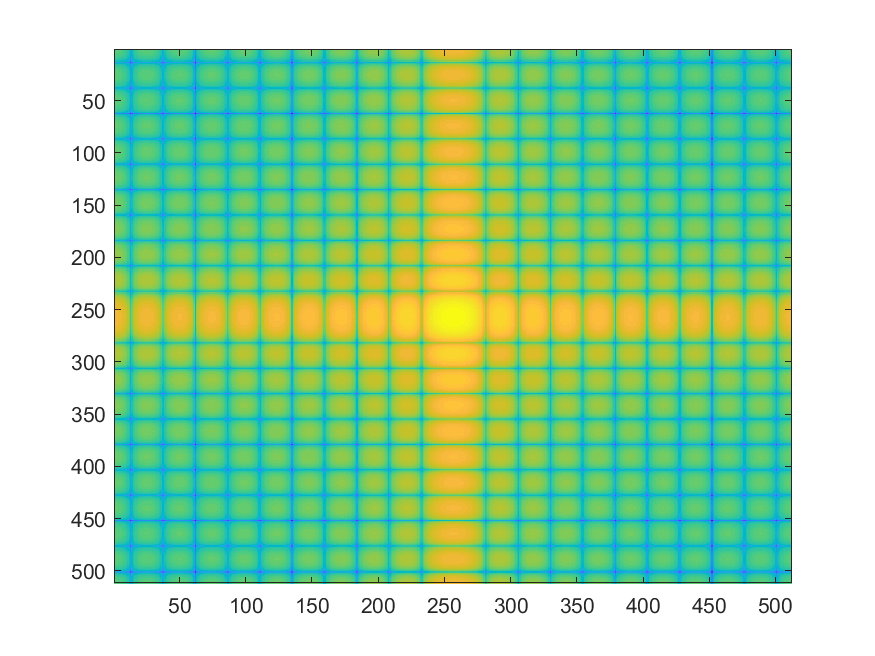
\includegraphics[scale=0.40]{figs/impl2_box2_spec.png}
}
\subfigure[Gaussian $31 \times 31$, $\sigma = 5$] {
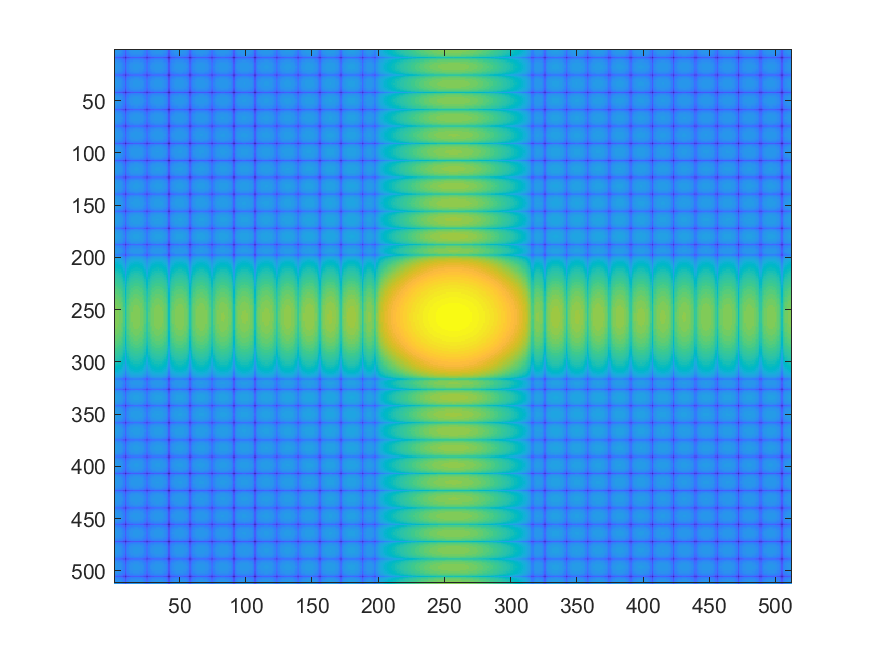
\includegraphics[scale=0.40]{figs/impl2_gauss1_spec.png}
}
\subfigure[Gaussian $55 \times 55$, $\sigma = 9$] {
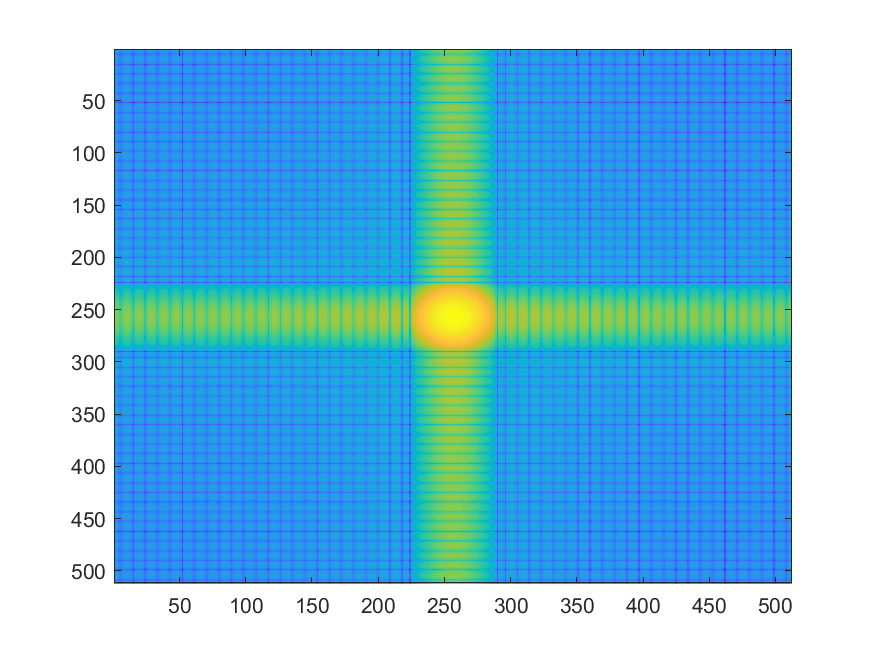
\includegraphics[scale=0.40]{figs/impl2_gauss2_spec.png}
}
\caption{Frequency spectrum of low pass filters.}\label{fig:impl2_spectrum}
\end{figure}

\textbf{검토사항} Box filter 의 경우 영상의 중앙에 pass band 와 비교할 때, stop band 의 ripple 이 거의 비슷한 수준의 magnitude 를 가진다는 것을 알 수가 있다. 반대로 Gaussian filter 의 경우에는 stop band 의 magnitude 가 pass band 에 비해서 굉장히 작다. 이를 통해서 box filter 가 gaussian filter 에 비해서 low pass 동작을 할 때 high-frequency 성분들을 상대적으로 덜 걸러낼 것이라고 예상을 할 수 있다.

Fig.\ref{fig:impl2_result}는 \code{chirp.tif} 영상에 각 filter 를 적용한 결과다.

\begin{figure}[H]
\centering
\subfigure[Box $11 \times 11$] {
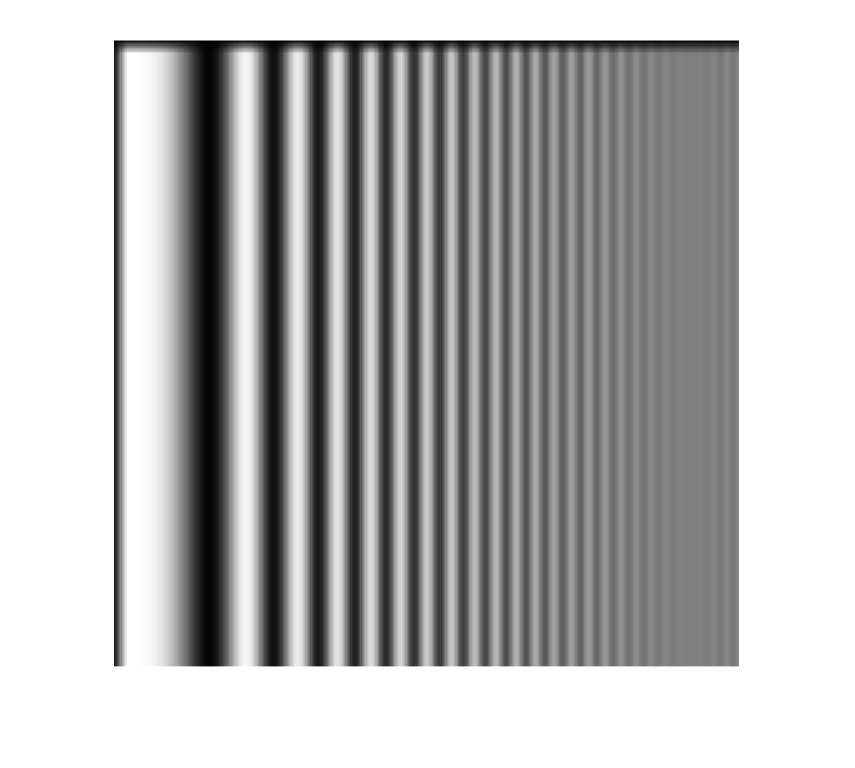
\includegraphics[scale=0.40]{figs/impl2_box1_result.png}
}
\subfigure[Box $21 \times 21$] {
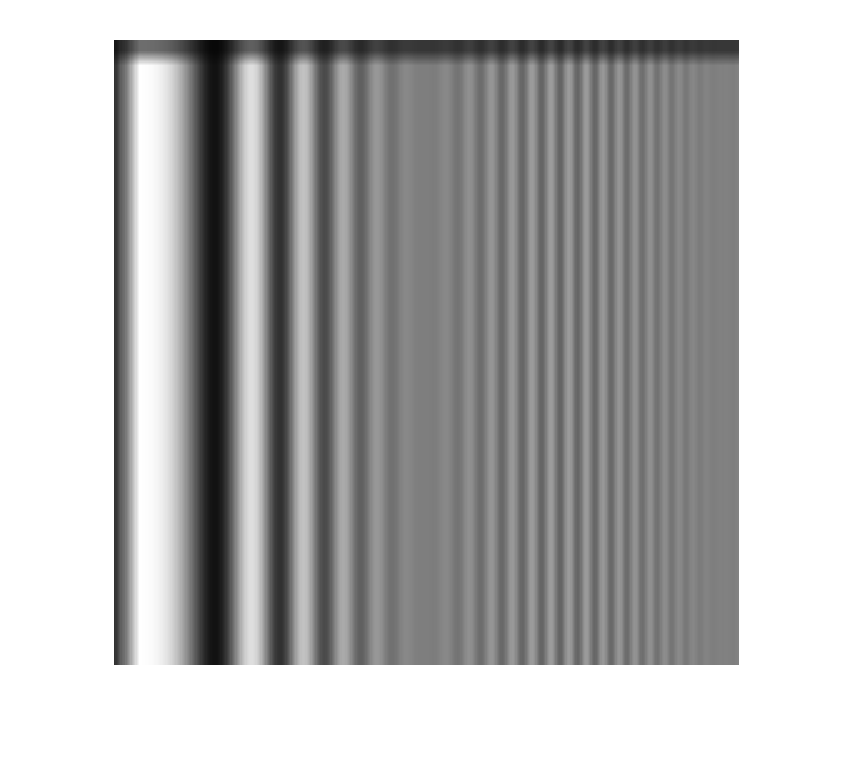
\includegraphics[scale=0.40]{figs/impl2_box2_result.png}
}
\subfigure[Gaussian $31 \times 31$, $\sigma = 5$] {
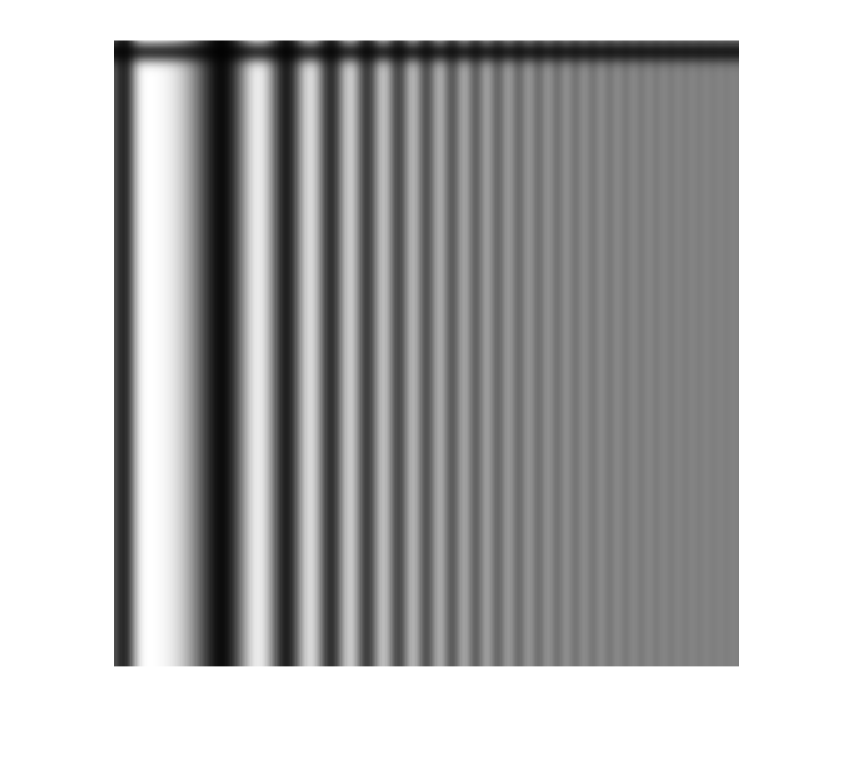
\includegraphics[scale=0.40]{figs/impl2_gauss1_result.png}
}
\subfigure[Gaussian $31 \times 31$, $\sigma = 5$] {
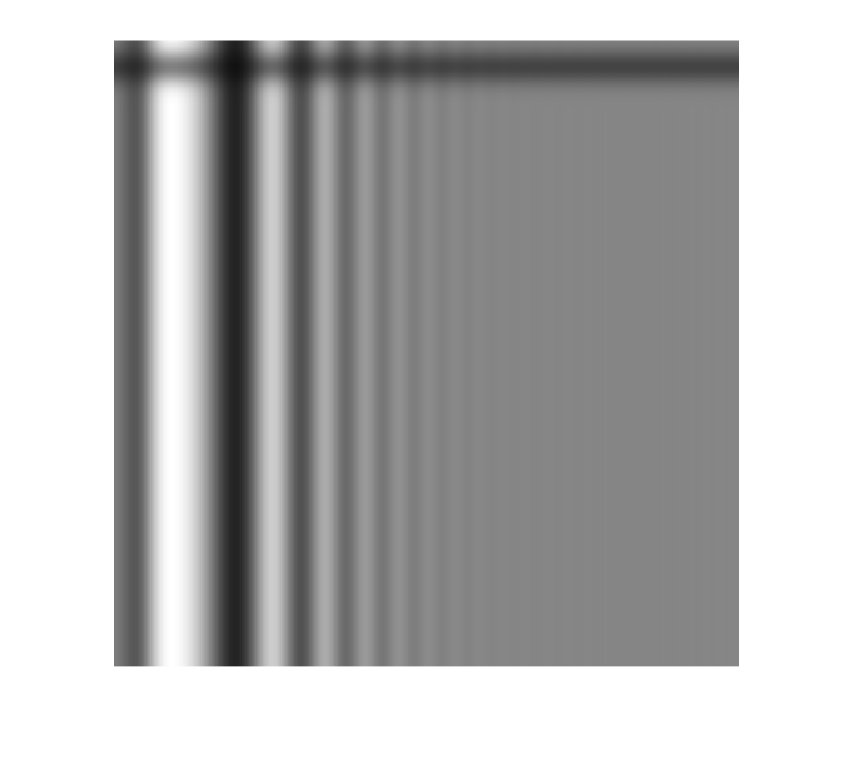
\includegraphics[scale=0.40]{figs/impl2_gauss2_result.png}
}
\caption{Result of appyling low pass filters on \code{chirp.tif}}\label{fig:impl2_result}
\end{figure}

이전에 예상했던대로, box filter 를 적용한 경우에 상대적으로 고주파 영역의 촘촘한 무늬들이 더 잘 보이는 것을 확인할 수 있다. 특히 $21 \times 21 $ 필터를 적용한 경우에는 일부 주파수 대역이 상대적으로 덜 attenuation 된 band pass 현상을 보인다. 이는 box filter 에서 강하게 나타나는 gibbs ringing 의 영향으로 추정해볼 수 있다.

\subsection{Implementation 3}
마지막으로 구현3 은 주기적인 현상을 보이는 노이즈가 섞인 이미지를, notch filter 를 이용해서 복원하는 것이다. 주어진 영상 \code{Astronaut.tif} 의 frequency spectrum 을 Fig.~\ref{fig:impl3_spectrum} 에서 보면, 세로로 강한 주파수 성분이 존재하는 것을 볼 수 있다. 이 부분의 band 를 reject 하는 notch filter 적용해서 (b) 와 같이 spectrum을 변형하였다. Fig.\ref{fig:impl3_result} 에서 filter 를 적용한 결과를 비교한 것을 볼 수 있다. 필터 적용 결과 상당부분 noise 가 제거된 것을 확인할 수 있다. 추출한 noise 는 원본 영상에서 보이는 주기적인 noise 와 거의 일치한다. Noise 가 굉장히 정확하게 제거되는 동시에 원본 영상에서 왜곡이 크게 발생하지 않는다. 이 점에서 frequency domain filtering 의 강력한 점을 느껴볼 수 있다.

\begin{figure}[H]
\centering
\subfigure[Original spectrum] {
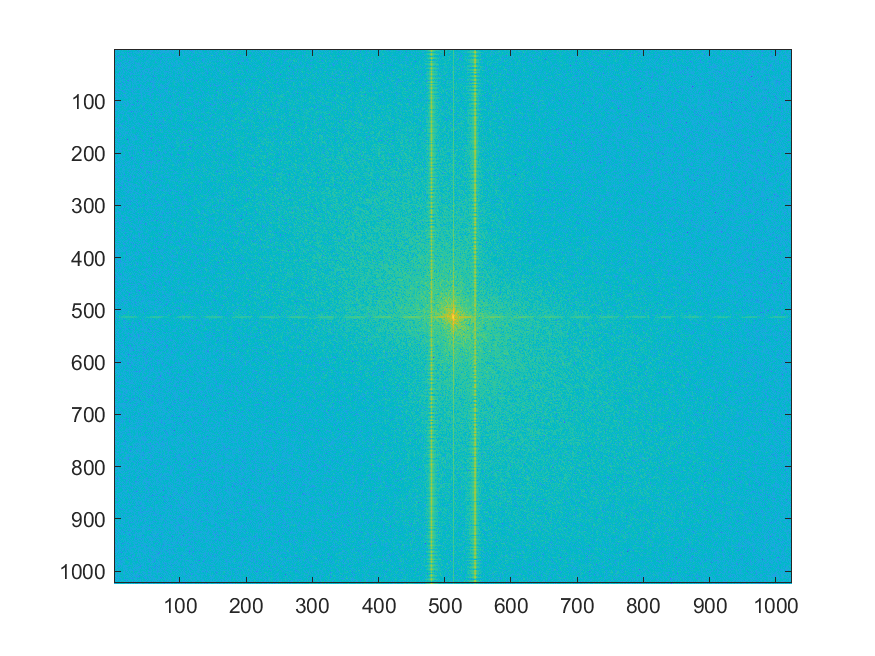
\includegraphics[scale=0.40]{figs/impl3_spectrum.png}
}
\subfigure[Filtered spectrum] {
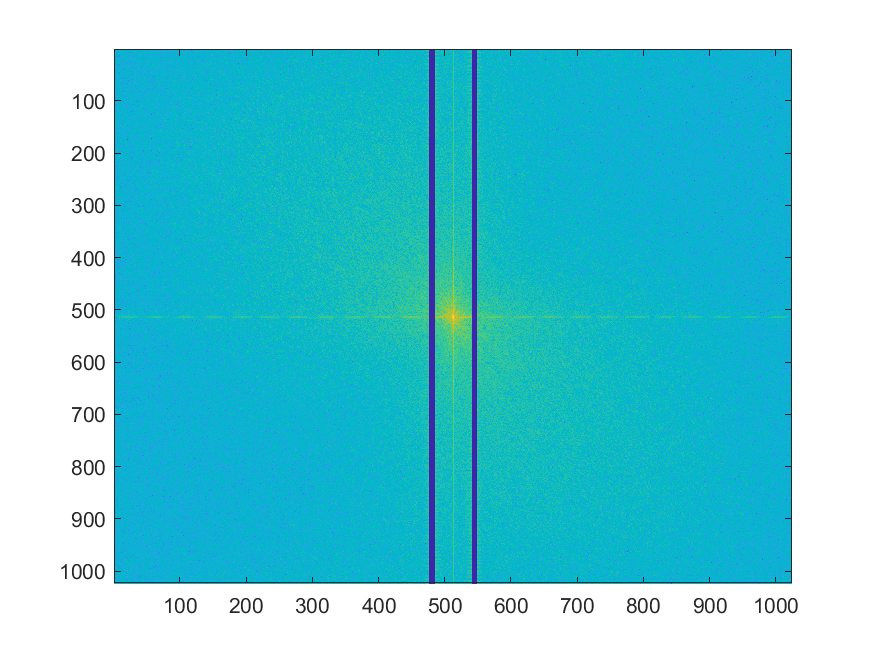
\includegraphics[scale=0.40]{figs/impl3_masked.png}
}
\caption{Original spectrum and the spectrum after applying the notch filter.}\label{fig:impl3_spectrum}
\end{figure}

\begin{figure}[H]
\centering
\subfigure[\code{Astronaut.png}] {
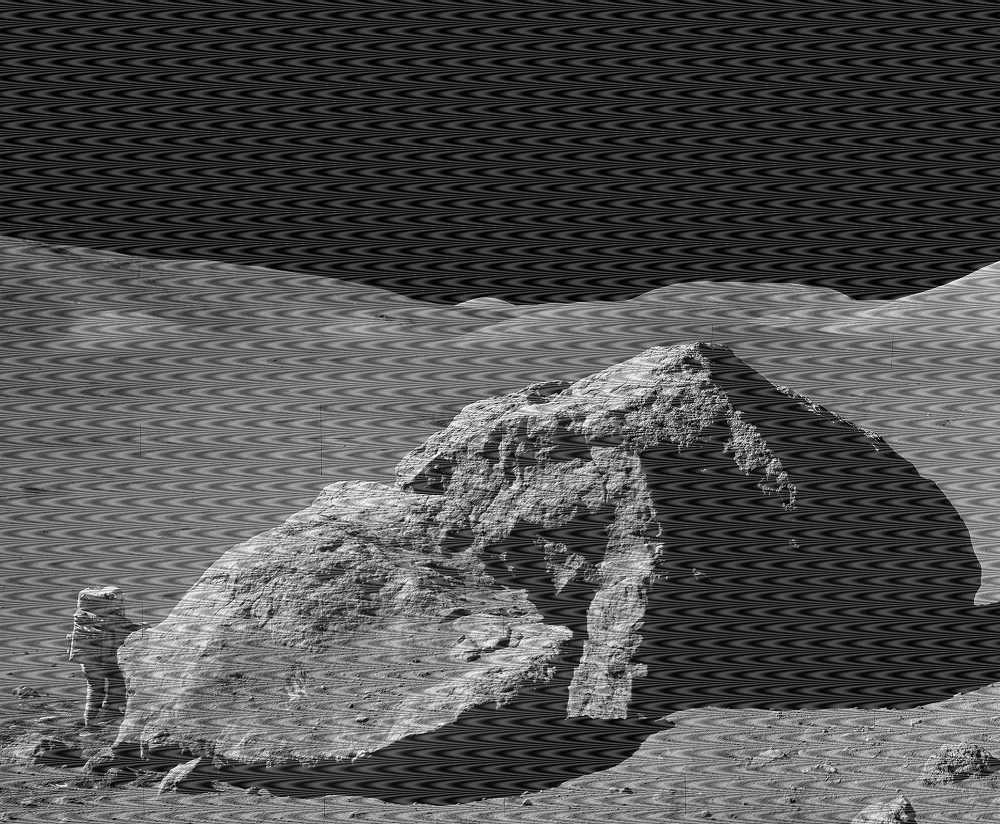
\includegraphics[scale=0.15]{figs/Astronaut.png}
}
\subfigure[Reconstructed] {
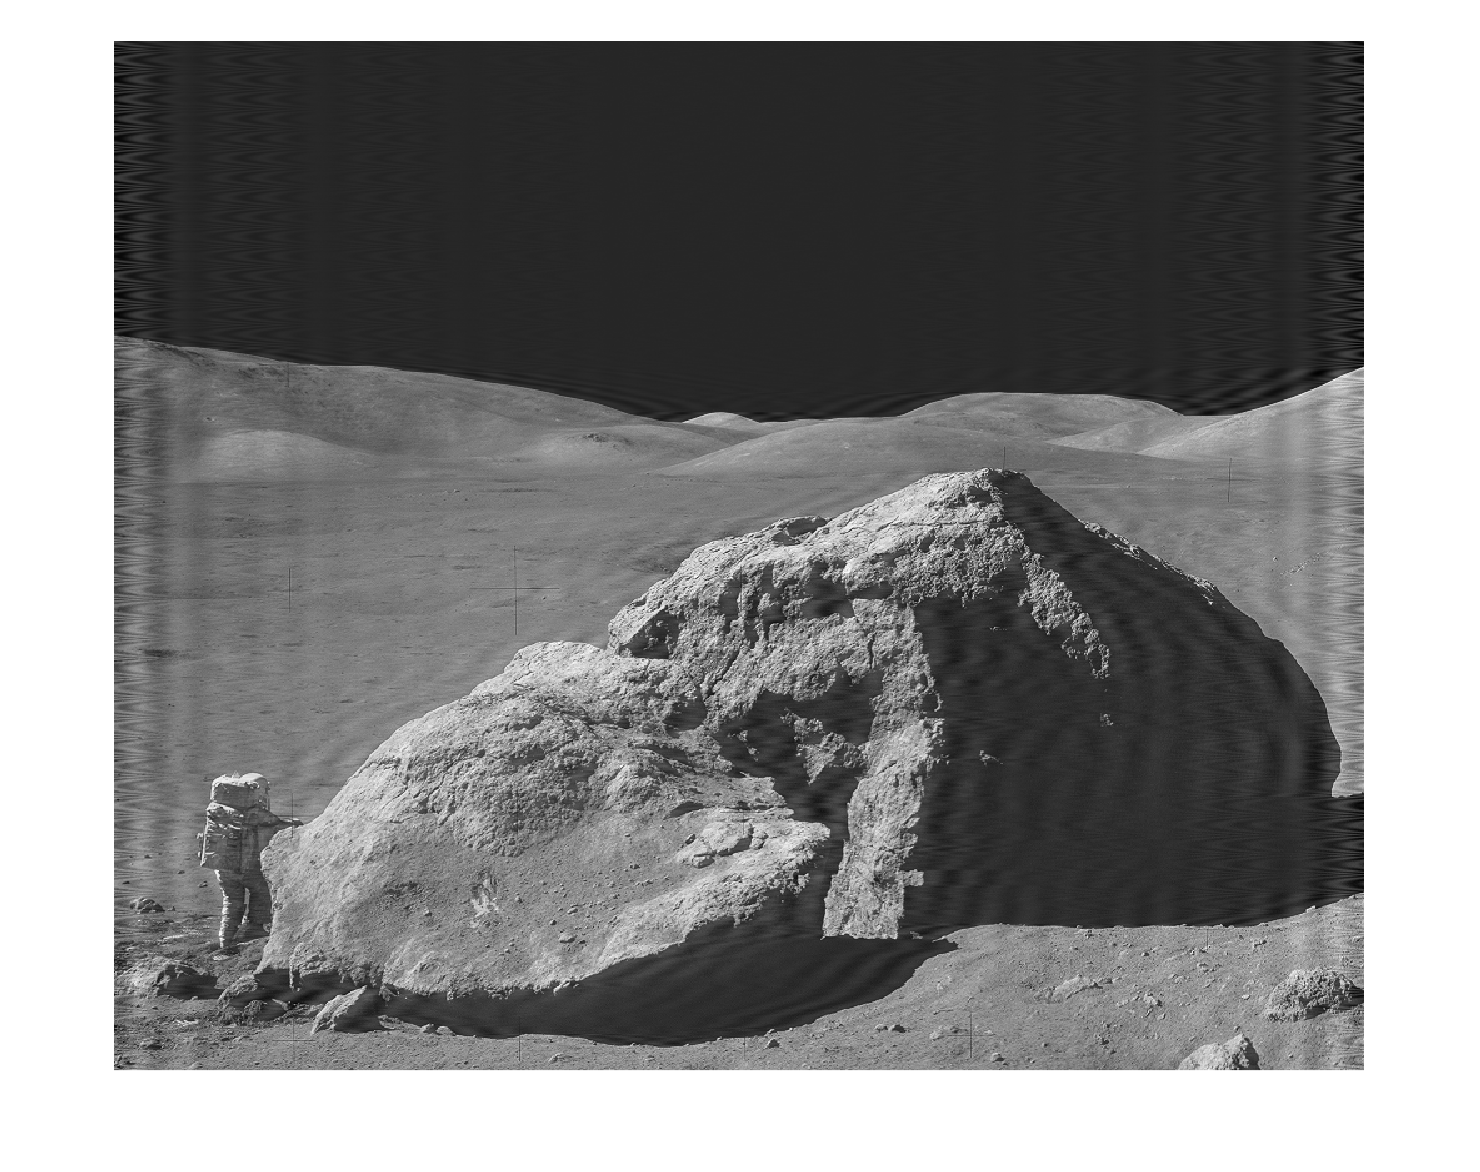
\includegraphics[scale=0.2]{figs/impl3_recon.png}
}
\subfigure[Noise] {
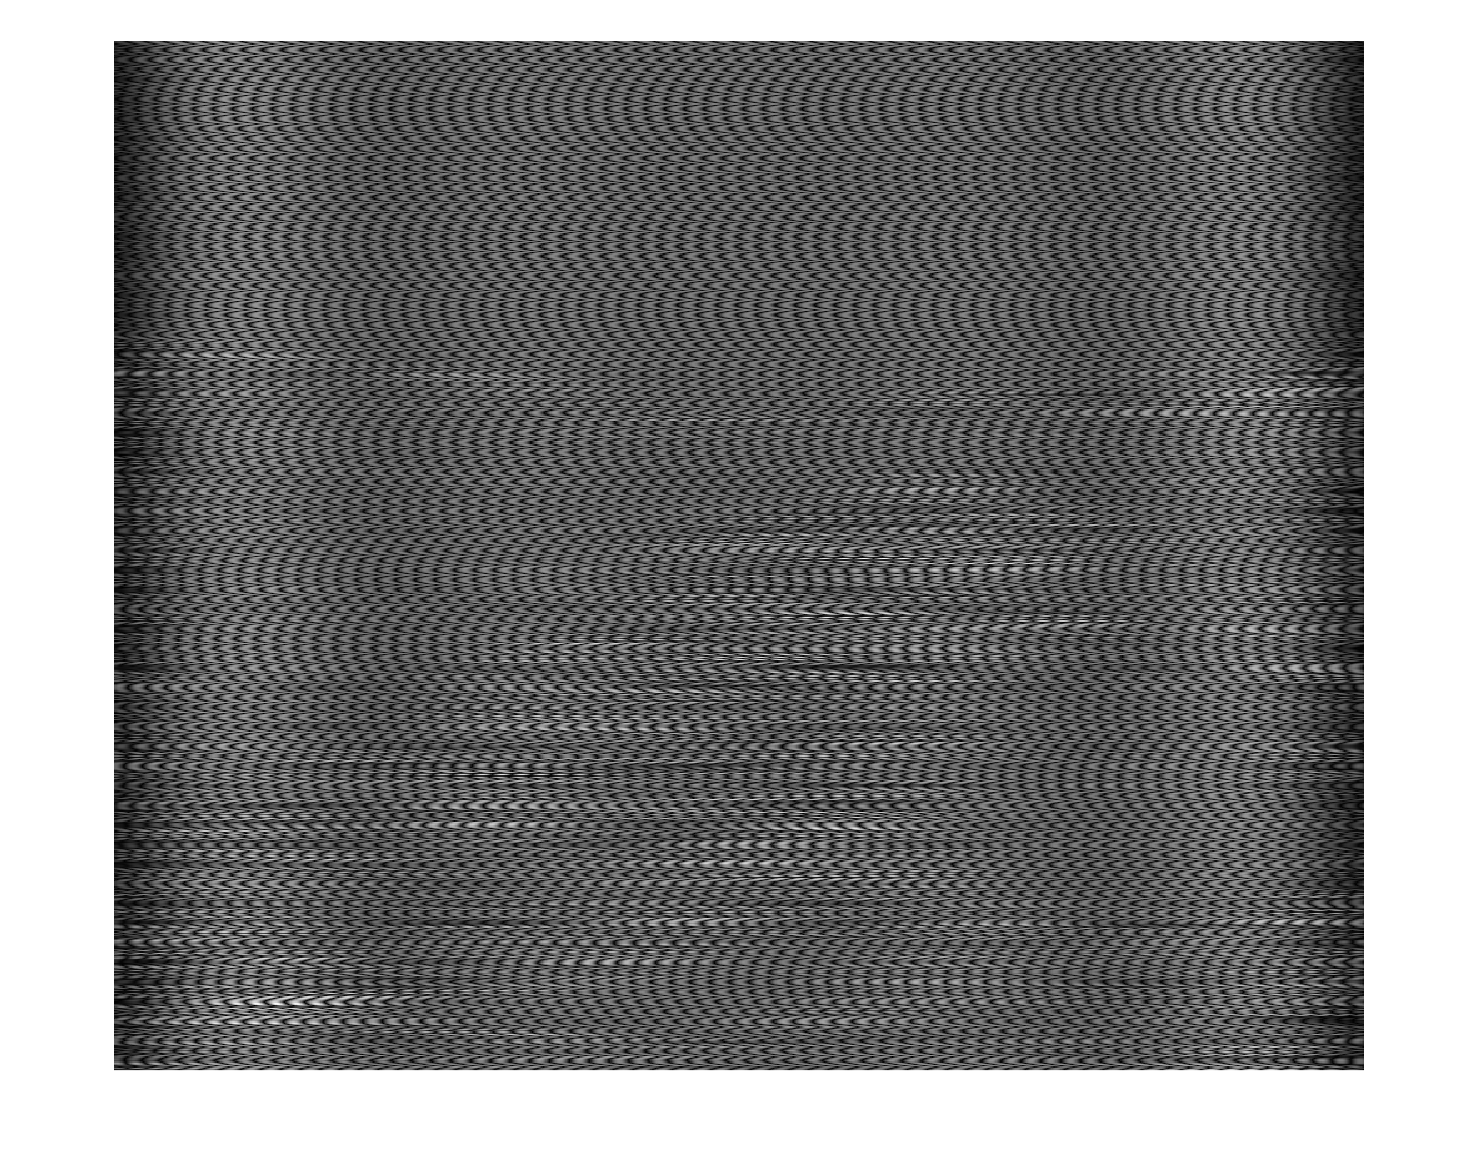
\includegraphics[scale=0.2]{figs/impl3_noise.png}
}
\caption{Reconstructed image and extracted noise using notch filter.}\label{fig:impl3_result}
\end{figure}

\section{Conclusion}
디지털 영상의 frequency domain analysis 를 통해서, frequency spectrum 과 phase angle 의 역할에 관해서 알아보았다. 또한 Box filter, Gaussian filter 와 같이 대표적인 Low-pass filter 들의 frequency spectrum 을 통해서 그 시각적으로 분석하였다. 마지막으로, 강한 주기성을 가진 노이즈를 notch filter 를 통해 제거하는 것을 해보았으며, 이를 통해 frequency domain filtering 의 효율성을 경험할 수 있었다.

\end{document}
